\documentclass[12pt,oneside]{fithesis2}
\usepackage[english]{babel}
\usepackage[utf8]{inputenc}
\usepackage[T1]{fontenc}
\usepackage[shortlabels]{enumitem}
\usepackage[
  scaled=0.86
]{berasans}
\usepackage[
  scaled=1.03
]{inconsolata}
\usepackage[
  plainpages = false,
  pdfpagelabels
]{hyperref}
\usepackage[autostyle]{csquotes}
\usepackage[super]{nth}
\usepackage{blindtext}
\usepackage{graphicx}
\usepackage{float}
\setlist[enumerate]{font=\bfseries}
\usepackage{listings}
\usepackage{color}
\thesislang{en}
\thesistitle{Information systems integration and process osptimization in a software company}
\thesissubtitle{Diploma Thesis}
\thesisstudent{Bc. Martin Jordán}
\thesiswoman{true}
\thesisfaculty{fi}
\thesisyear{Winter 2021}
\thesisadvisor{Ing. Leonard Walletzký, PhD.}
\graphicspath{{images/}}


\makeatletter
\usepackage{color}
\definecolor{lightgray}{rgb}{0.95, 0.95, 0.95}
\definecolor{darkgray}{rgb}{0.4, 0.4, 0.4}
%\definecolor{purple}{rgb}{0.65, 0.12, 0.82}
\definecolor{editorGray}{rgb}{0.95, 0.95, 0.95}
\definecolor{editorOcher}{rgb}{1, 0.5, 0} % #FF7F00 -> rgb(239, 169, 0)
\definecolor{editorGreen}{rgb}{0, 0.5, 0} % #007C00 -> rgb(0, 124, 0)
\definecolor{orange}{rgb}{1,0.45,0.13}		
\definecolor{olive}{rgb}{0.17,0.59,0.20}
\definecolor{brown}{rgb}{0.69,0.31,0.31}
\definecolor{purple}{rgb}{0.38,0.18,0.81}
\definecolor{lightblue}{rgb}{0.1,0.57,0.7}
\definecolor{lightred}{rgb}{1,0.4,0.5}
\usepackage{upquote}
\usepackage{listings}
% CSS
\lstdefinelanguage{CSS}{
  keywords={color,background-image:,margin,padding,font,weight,display,position,top,left,right,bottom,list,style,border,size,white,space,min,width, transition:, transform:, transition-property, transition-duration, transition-timing-function},	
  sensitive=true,
  morecomment=[l]{//},
  morecomment=[s]{/*}{*/},
  morestring=[b]',
  morestring=[b]",
  alsoletter={:},
  alsodigit={-}
}

% JavaScript
\lstdefinelanguage{JavaScript}{
  morekeywords={typeof, new, true, false, catch, function, return, null, catch, switch, var, if, in, while, do, else, case, break},
  morecomment=[s]{/*}{*/},
  morecomment=[l]//,
  morestring=[b]",
  morestring=[b]'
}

\lstdefinelanguage{HTML5}{
  language=html,
  sensitive=true,	
  alsoletter={<>=-},	
  morecomment=[s]{<!-}{-->},
  tag=[s],
  otherkeywords={
  % General
  >,
  % Standard tags
	<!DOCTYPE,
  </html, <html, <head, <title, </title, <style, </style, <link, </head, <meta, />,
	% body
	</body, <body,
	% Divs
	</div, <div, </div>, 
	% Paragraphs
	</p, <p, </p>,
	% scripts
	</script, <script,
  % More tags...
  <canvas, /canvas>, <svg, <rect, <animateTransform, </rect>, </svg>, <video, <source, <iframe, </iframe>, </video>, <image, </image>, <header, </header, <article, </article
  },
  ndkeywords={
  % General
  =,
  % HTML attributes
  charset=, src=, id=, width=, height=, style=, type=, rel=, href=,
  % SVG attributes
  fill=, attributeName=, begin=, dur=, from=, to=, poster=, controls=, x=, y=, repeatCount=, xlink:href=,
  % properties
  margin:, padding:, background-image:, border:, top:, left:, position:, width:, height:, margin-top:, margin-bottom:, font-size:, line-height:,
	% CSS3 properties
  transform:, -moz-transform:, -webkit-transform:,
  animation:, -webkit-animation:,
  transition:,  transition-duration:, transition-property:, transition-timing-function:,
  }
}

\lstdefinestyle{htmlcssjs} {%
  % General design
%  backgroundcolor=\color{editorGray},
  basicstyle={\footnotesize\ttfamily},   
  frame=b,
  % line-numbers
  xleftmargin={0.75cm},
  numbers=left,
  stepnumber=1,
  firstnumber=1,
  numberfirstline=true,	
  % Code design
  identifierstyle=\color{black},
  keywordstyle=\color{blue}\bfseries,
  ndkeywordstyle=\color{editorGreen}\bfseries,
  stringstyle=\color{editorOcher}\ttfamily,
  commentstyle=\color{brown}\ttfamily,
  % Code
  language=HTML5,
  alsolanguage=JavaScript,
  alsodigit={.:;},	
  tabsize=2,
  showtabs=false,
  showspaces=false,
  showstringspaces=false,
  extendedchars=true,
  breaklines=true,
  % German umlauts
  literate=%
  {Ö}{{\"O}}1
  {Ä}{{\"A}}1
  {Ü}{{\"U}}1
  {ß}{{\ss}}1
  {ü}{{\"u}}1
  {ä}{{\"a}}1
  {ö}{{\"o}}1
}
%
\lstdefinestyle{py} {%
language=python,
literate=%
*{0}{{{\color{lightred}0}}}1
{1}{{{\color{lightred}1}}}1
{2}{{{\color{lightred}2}}}1
{3}{{{\color{lightred}3}}}1
{4}{{{\color{lightred}4}}}1
{5}{{{\color{lightred}5}}}1
{6}{{{\color{lightred}6}}}1
{7}{{{\color{lightred}7}}}1
{8}{{{\color{lightred}8}}}1
{9}{{{\color{lightred}9}}}1,
basicstyle=\footnotesize\ttfamily, % Standardschrift
numbers=left,               % Ort der Zeilennummern
%numberstyle=\tiny,          % Stil der Zeilennummern
%stepnumber=2,               % Abstand zwischen den Zeilennummern
numbersep=5pt,              % Abstand der Nummern zum Text
tabsize=4,                  % Groesse von Tabs
extendedchars=true,         %
breaklines=true,            % Zeilen werden Umgebrochen
keywordstyle=\color{blue}\bfseries,
frame=b,
commentstyle=\color{brown}\itshape,
stringstyle=\color{editorOcher}\ttfamily, % Farbe der String
showspaces=false,           % Leerzeichen anzeigen ?
showtabs=false,             % Tabs anzeigen ?
xleftmargin=17pt,
framexleftmargin=17pt,
framexrightmargin=5pt,
framexbottommargin=4pt,
%backgroundcolor=\color{lightgray},
showstringspaces=false,      % Leerzeichen in Strings anzeigen ?
}%
%
\makeatother


\begin{document}
  \FrontMatter
    \ThesisTitlePage
    \begin{ThesisDeclaration}
      \DeclarationText
      \AdvisorName
    \end{ThesisDeclaration}
    \begin{ThesisThanks}
      I would like to thank my supervisor Ing. Leonard Walletzký, PhD. for guidance and valuable professional and personal insights. Secondly, I would like to thank my wife, Jana Jordánová, who has been a tremendous mental support throughout all of my studies. This thesis would not be possible without the opportunity to work for the chosen company that has been given to me by Mr. Ivan Bradáč. \,\dots
    \end{ThesisThanks}
    \begin{ThesisAbstract}
      This thesis deals with information systems integration and analysing, modelling and optimizing processes in the financial department. The subject is to integrate two otherwise not compatible systems and create an application that would automate a specific process. These goals stem from specific needs of a private company, therefore we examine the current state and gather project requirements. Based on the collection of requirements we propose and implement a solution. Finally, we evaluate the added value of our solution.
    \end{ThesisAbstract}
    \begin{ThesisKeyWords}Process Automation, Systems integration, Finance, European Union funding programmes
    \end{ThesisKeyWords}
    \tableofcontents
  
  \MainMatter
    \chapter{Introduction}
    When assessing whether a company is successful or not, we can look at many different metrics ranging from market share, through the number of products sold over a specific period of time all the way to customer satisfaction. However, there is one metric that stands above all - financial success. After all, the end goal of every company is to generate, continually increase and maximize profit over a sustained period of time.
    \par
    In the early stages, it can be difficult for a company to achieve positive financial results. To accelerate growth, companies are constantly searching for ways to acquire cheap capital, optimize their processes and reduce costs.
    \par
    To drive innovation, European Union is offering funding programmes (sometimes also called calls) to companies in various areas of expertise. To be able to acquire these funds, firms must comply to a strict set of rules set by the European Commission.
    \par
    Alternatively, small companies turn to bigger players in the same space to sell them a stake in the company for a financial injection. This can create many different challenges, such as an incompatibility of certain systems the companies are using.
    \par
    The main idea of this thesis is to automate certain tasks to remove unnecessary operational overhead from company employees.
    \par
    The system is designed exclusively for a private company, whose area of expertise is developing software for Smart TVs.
    \newpage
    \section{Thesis goals}
    This thesis aims to solve the two problems described above. Firstly, it is to provide the company with means of reducing costs through automating the process of calculating specific indicator that is needed to determine the eligibility for the funding programmes. Secondly, it is to reduce the workload on daily operation by integrating two separate systems.
    \section{Thesis structure}
    The content of this paper is divided into seven chapters. The opening chapter serves as an introduction to better understand the domain within which this thesis operates. It describes the EU funding programmes and presents their motivation and goals in general. Furthermore, it introduces important concepts such as company size, job position relevance and annual work unit. The next chapter is dedicated to presenting the methodology of the thesis. The chapter after that analyzes the processes and presents the requirements for automating said processes. Following that, the optimized processes are presented together with some of the technologies used. Finally, the last chapter contains the implementation and deployment details.
    \chapter{Understanding the domain}
    In the following paragraphs, the domain of this thesis is presented. The purpose of this is to familiarize the reader with the domain so they can better understand the added value this thesis provides.
    \par
    The conducted research is designed to examine the funding programmes, to provide an explanation as to why they are offered by the European Union (EU) in the first place and to identify their limitations and analyze their rules and conditions in order to be able to create a software solution that would help achieve the thesis goals. Also, the reasons why the company is taking part in the selected funding programmes are presented here.
    \par
    The analysis of the limitations and rules is achieved by collecting information from various different sources, including EU regulations, web sites and the Czech Civil Code as well as by interviewing the stakeholders. From a software engineering perspective, this process is called the Business Analysis.\footnote{"Business Analysis (BA) is the practice of enabling change in an organizational context, by defining needs and recommending solutions that deliver value to stakeholders."\cite{business-analysis}}
    \par
    In the first section, the EU funding programmes are introduced. Here, general motivation for the funding programmes is presented. After that, the terms medium-sized, small and micro enterprise together with the staff headcount and relevant and non-relevant job positions are defined. From these, the annual work unit (AWU) indicator is then derived. Furthermore, the specific conditions a company has to adhere to in order to be eligible. Finally, there is information as to why the company is applying for the specific programmes. 
    \section{EU funding programmes}
    The EU funding programmes are funding opportunities created by the European Commission to help micro, small and medium-sized enterprises (SMEs) gain access to cheap capital through grants, loans and guarantees. The companies can also bid for contracts to provide goods and services.
    The specific project this thesis deals with is: "The company Mautilus, s.r.o. is implementing the project \textit{"New Apps Development in co. Mautilus"}, the goal of which is to develop multi-screen OTT (Over-the-top) applications designated for wide range of platforms that allow to watch video content." \cite{mau-eu-subsidy}
    \subsection{Motivation for funding programmes}
    The Czech Civil Code considers: "A person who, on his own account and responsibility, independently carries out a gainful activity in the form of a trade or in a similar manner with the intention to do so consistently for profit is considered, with regard to this activity, to be an entrepreneur."\cite{entrepreneur-law}
    \par
    The quintessential part: "...carries out a gainful activity in the form of a trade or in a similar manner with the intention to do so consistently for profit..."\cite{entrepreneur-law} ties in well with the concept of financial leverage. \footnote{"Financial leverage, also known as leverage or trading on equity, refers to the use of debt to acquire additional assets."\cite{financial-leverage}} This concept is often used to accelerate growth.
    \par
    While it is entirely possible for a company to grow organically, it would be pointless to argue against obtaining cheap capital. Even more so, when the company does not have to accrue debt in order to acquire the resources. Therefore, funding programmes make perfect sense for SMEs, because they provide reasonable amounts of fairly accessible capital, while having no impact on the distribution of the company share.
    \newline\newline
    In the document: "Political Guidelines for the next European Commission" from \nth{15} July 2014, Jean-Claude Juncker, a Candidate for President of the European Comission stated the following: \blockquote{"Jobs, growth and investment will only return to Europe if we create the right regulatory environment and promote a climate of entrepreneurship and job creation. We must not stifle innovation and competitiveness with too prescriptive and too detailed regulations, notably when it comes to SMEs. They are the backbone of our economy, creating more than 85\% of new jobs in Europe and we have to free them from burdensome regulation."\cite{juncker-political-guidelines}}
    In the year 2020, maybe more than ever before, we have seen that small businesses are a vital wheel in such a delicate and fragile machine that our economy undoubtedly is. It is not the purpose of this thesis to defend, nor argue against monetary policies and massive fiscal stimulus that we have seen in the past year. If anything, it is to demonstrate that European funds are being put to a good use. These lines portray the appetite European Union has for growth and innovation. Reading this, we can see a clear indication that growth, overall well being and abundance are the main motivators behind these funding calls.
    \newline\newline
    Also, in the same document, Mr. Juncker wrote: \blockquote{"Beyond that, I will leave other policy areas to the Member States where they are more legitimate and better equipped to give effective policy responses at national, regional or local level, in line with the principles of subsidiarity and proportionality. I want a European Union that is bigger and more ambitious on big things, and smaller and more modest on small things."\cite{juncker-political-guidelines}}
    From the first part, we can see that Mr. Juncker has a genuine interest in enabling the Member States invest in their future. He then solidifies this by empowering them to take ownership of their local policies. He does all of this while maintaining a sober approach to such a delicate topic that is public resources.
    
    To summarize, we can say that we see a genuine effort towards allocating public money in a fair and reasonable manner that is sustainable over the long term and helps small businesses grow into flourishing enterprises that solve real world problems. Without a doubt, this is a good enough motivation for such funding programmes to exist.
    \subsection{Company size}
    \noindent
    According to the Commision regulation No.651/2014 \cite[page~70]{eu-commision-regulation} issued by the European Comission, the companies are divided into three categories according to the number of employees and annual turnover:
    \begin{enumerate}
        \item Medium-sized enterprise
        \newline\newline
        Within the SME category, a medium-sized enterprise must have fewer than 250 employees and have an annual turnover not exceeding EUR 50 million, and/or an annual balance sheet not exceeding EUR 43 million.
        \item Small enterprise
        \newline\newline
        A small enterprise is defined as an enterprise which employs fewer than 50 persons and whose annual turnover and/or annual balance sheet total does not exceed EUR 10 million.
        \item Micro-enterprise
        \newline\newline
        A micro-enterprise is defined as an enterprise which employs fewer than 10 persons and whose annual turnover and/or annual balance sheet total does not exceed EUR 2 million.
    \end{enumerate}
    These figures apply to individual companies only. A small company might not qualify for SME status if it has significant additional resources because it is part of a larger group. \cite{eu-commision-regulation}
    It is imperative for a company applying for a funding programme to fall into one of these three categories. If they don't, they are rejected. Our company falls into the small enterprise category.
    \subsection{Job position relevance}
    When applying for a programme, the relevance of a job position with respect to the project needs to be taken into account. Non-relevant employees are not accounted for in the AWU calculation. Nevertheless, it is useful to have this information.
    
    It is also important to note that only employees working in the office that is listed in the application can be taken into account.\cite[page~30]{czech-rules}
    \subsection*{Relevant (R)}
    Employees, whose qualification and job are directly related to the project in question. (i.e. developers in our case)\cite[page~30]{czech-rules}
    \subsection*{Non-relevant (N)}
    All other employees fall into this category. (i.e. management, sales, accountants etc.)\cite[page~30]{czech-rules}
    \subsection{Annual work unit (AWU)}
    We have established that in order to be eligible for funding, a company has to have a certain amount of employees. Knowing only this would not suffice, as we need to take into account the time our employees have really worked. To enable this fine-grained distinction, European Union introduces the AWU.
    \newline\newline
    The European Comission defines the AWU as:
    \blockquote{"...the number of persons who worked full- time within the enterprise in question or on its behalf during the entire reference year under consideration. The work of persons who have not worked the full year, the work of those who have worked part-time, regardless of duration, and the work of seasonal workers are counted as fractions of AWU."\cite[page~71]{eu-commision-regulation}}
    In practice, this means an employee's contract is represented on a scale from 0 to 1 where 0 means they are either currently not employed (i.e. an employee who resigned) or they have been on an unpaid leave. Conversely, 1 means they are working full time.
    
    This means that the work of employees who have not worked the full year, the work of those who have worked part-time, regardless of the duration and the work of seasonal workers are counted as fractions of AWU.
    
    When taking into con
    \newline\newline The staff consists of:
    \begin{enumerate}[A)]
        \item employees;
        \item persons working for the enterprise being subordinated to it and deemed to be employees under national law; 26.6.2014 EN Official Journal of the European Union L 187/71;
        \item owner-managers;
    \end{enumerate}
    Apprentices or students engaged in vocational training with an apprenticeship or vocational training contract are not included as staff. The duration of maternity or parental leaves is not counted. \cite{eu-commision-regulation}
    \section{Systems integration}
    Merging two companies together is always a complicated process that can take months or even years to fully complete. At each point in time, there are too many moving parts for a small group of executives to keep up with. Beyond a certain complexity threshold, the ability to recognize inefficiencies that could arise from such process can be non-existent. In a company of almost any size, as long as there are two or more information systems, a possibility exists that there will be a need to use data from one system in the other.
    
    \textit{Here will be more information about systems integration in general. How they are usually handled and how we are planning on approaching the problem.}
    \chapter{Methodology}
    After the initial interviews with the stakeholders had been concluded, it was proposed that agile development methodology is used. This seemed like a good idea in the beginning, as the company already used scrum as their workflow for other projects. However, shortly thereafter it became apparent that scrum would introduce more complexity rather than help streamline the workflow. Because of this, it was decided that the prototyping workflow is used. That is, at least for the scope of the project as defined by this thesis. This enabled us to maintain high level of flexibility while maintaining low level of operational overhead.
    
    The first prototype was created from an open-source template and deployed through a personal AWS account. It was used to verify whether or not it would be effective to use chosen technologies. After presenting this prototype to the stakeholders, the technologies were evaluated as feasible and the project was approved to use company infrastructure. Since the first prototype was tied to a personal account, it was then discarded.
    
    Since this project has been in progress for some time, it has also been affected by new additions to the AWS ecosystem. This is why a second prototype was created. Here, user creation and login functionality has been improved. With the new Amplify Admin UI, it is now easier to create and approve users. Previously the approval had to be done through the command line.
    \chapter{Analysis}
    This chapter deals with analysing the problems arising in the company that led to creating this thesis. First, we look at the current approaches to solving these problems. Then, we  ...
    
    will contain models of the processes made by the financial department before and after this solution has been implemented.
    Since there is no need to 
    \section{WBS}
    To successfully manage software development it is essential that all of the tasks are well defined, assigned, scheduled and controlled. The most commonly used technique to achieve this is the process of systematically organizing tasks into a form called the Work breakdown structure (WBS). It contains all of the tasks to be accomplished during the project and is organized in a hierarchical structure.
    \par
    The WBS typically defines the whole system to be developed, produced, tested, deployed, and supported, including hardware, software, services, and data. In other words, it defines a framework within which the project is to be implemented. \cite{systems-engineering}
    \section{Current state}
    In this section, we will describe the processes and create their models with BPMN.\footnote{"Business Process Model and Notation is the standard for business processes diagrams. It is intended to be used directly by the stakeholders who design, manage and realize business processes, but at the same time be precise enough to allow BPMN diagrams to be translated into software process components. BPMN has an easy-to-use flowchart-like notation that is independent of any particular implementation environment."\cite{bpmn}} The following lines are dedicated to exploring how the processes are currently being carried out, what are some their 
    \subsection{Calculating the AWU}
    In the current state, in order to calculate the AWU, an employee has to manually export the data from accounting systems. Then, based on worker capacity, a decision has to be made whether or not to calculate the AWU internally, or outsource it to an external company. Regardless of which route we take, we always end up with a person having to manually copy data from one table to another in order to calculate the AWU. As such, we can say that both of these options are sub-optimal, as one carries workload overhead and the other creates increased costs. Both of which could be put to a better use, if we were to automate at least some parts of the process.
    
    The following figure shows the process of calculating the AWU prior to creation of this thesis. It is clear that there are tasks which can be automated. We will focus on automating the task: "Calculate AWU", as we can achieve the highest time and costs savings.
    \begin{figure}[htp]
        \centering
        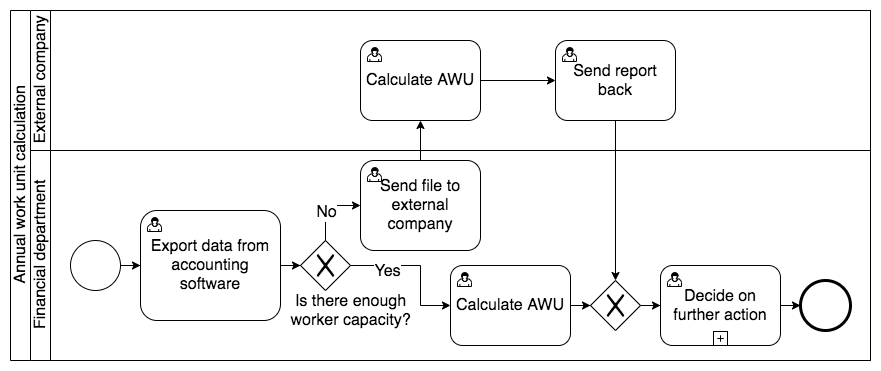
\includegraphics[width=\textwidth]{before_automation.png}
        \caption{Process before automation}
        \label{fig:before_automation}
    \end{figure}
    
    ---From this diagram it is apparent that there are steps that can be optimized and or entirely removed. In this thesis, we are going---
    
    \subsection{Systems integration}
    This section describes the process of requesting time off and introduces the subsequent problem created by using two separate systems for handling time reporting. The first system, BambooHR is used for requesting time off. The second one, Tempo Timesheets is used to keep track of how employees spend their time. This data is then used for invoicing and other financial purposes. To accommodate for efficient planning, however, this data has to always be in sync.
    
    From an employee's or manager's perspective, the process of requesting time off is fairly straightforward and does not require any steps that would be much of an issue when it comes to time spent on the tasks. The problem becomes apparent when the need arises to transfer this data to a different system. After time off has been approved by the manager, a worker in the HR department receives an email notification. They then have to go and manually input this data into another system. Moreover, they have to update this data even when a request has been approved, but then subsequently removed due to some unexpected reason. In a sense, the assistant is acting as a synchronizing agent between the two systems.
    
    \begin{figure}[H]
        \centering
        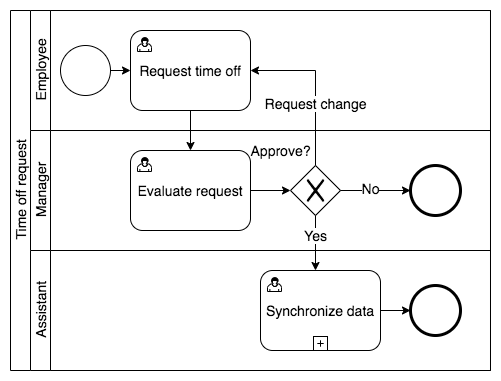
\includegraphics[width=\textwidth]{before_sys_integration.png}
        \caption{Process before system integration}
        \label{fig:before_sys_integration}
    \end{figure}
    The company wants to be able to automate this process in order to save time and reduce expenses. This can be done by using the application's public APIs.
    \newline\newline
    Across both systems, the company is using four types of leaves:
    \begin{enumerate}
        \setlength\itemsep{0em}
        \item Holiday leave
        \item Sick leave
        \item Birthday leave
        \item Special leave
    \end{enumerate}
    It is important that we keep these in mind, as they are the deciding factor for the solution we are eventually going to use. These types come into play later in the process, when accounting is being done. Hence, we cannot simply merge them into one leave.
    
    For each time off that has been 
    
    Once approved, the time off can still be deleted by the manager, as if it were never even requested.
    
    
    \section{Requirements analysis}
    Requirements analysis is the process of identifying the "whys" of all requirements in terms of needs and constraints. It serves to clarify the requirements of what the system must do, how well it must do it and what are the constraints it must fit.\cite{systems-engineering}
    
    In our current state analysis, we have concluded that we need to find a way of automating the task of calculating the AWU. To do this, we propose to create a web application that would fill all of the requirements described in the requirements analysis. We will now have a look at how we can implement the application to fulfill the functional requirements
    \subsection{Functional requirements}
    
    The following list of requirements has been derived from the interviews with the stakeholders.
    \begin{itemize}
        \item Login
        \item Reset password
        \item Upload a .xlsx file with data
        \item View computed AWU data
    \end{itemize}
    The user credentials are created by the administrator, hence there is no need for sign-up functionality.

    
    \subsection{Non-functional requirements}
    As the application deals with financial data, there are strong security requirements.
    \begin{itemize}
        \item The application must use some form of authentication
        \item The application must be available only through a VPN from company office
        \item Database can not be publicly available
        \item Any API can not be publicly available and must use authentication
    \end{itemize}
    Security
    
    
    
    \section{Solutions for systems integration}
    Tady bude popsaná integrace včetně typů volna
    
    For this integration, we are looking to 
  
    First, we will have a look at some of the solutions that are currently available in the market and determine whether or not they are viable for our use case. To do this, we used Google search to look for the term: "Tempo Timesheets BambooHR integration". We investigated the following list of services:
    \begin{itemize}
        \setlength\itemsep{0em}
        \item blendr.io 
        \item zapier
        \item BambooHR Integration for Jira
    \end{itemize}
    After reviewing these products, we came to the conclusion that the first two would not be viable options. Blendr \cite{blendr} Zapier does provide a trigger for new time off, however, there is no way of dealing with the type of the request afterwards. Moreover, there was no action that would correspond to our requirement of adding time to specific ticket.\cite{zapier}
    
    \subsection*{BambooHR Integration for Jira}
    While there is a wide variety of solutions for API integrations, they tend to be very generic and provide limited options for customization. The closest we could get with an out of the box solution was to use plugin for Jira called: "BambooHR Integration for Jira" developed by New Verve Consulting.
    
    When we compare these findings with the requirements for this integration, we  to the decision to create our own solution.
    
    \subsection*{Tempo Timesheets API}
    the suite of project management tools JIRA by Atlassian is used.
    Tady krátce představíme tempo sheets
    Poté ukážeme část api, kterou bychom využili při integraci
    \subsection*{BambooHR API}
    Tady představíme BambooHR a ukážeme, kterou část API bychom využili
    BambooHR is all-in-one HR software made for small and medium businesses. The software makes it easy to collect, maintain, and analyze employee data, on-board new employees, manage compensation, and develop your company culture.\cite{bambooHR}
    
    One of the features this software provides is 
    
    In BambooHR, we are looking for: 
    
    In the documentation, we were looking for an endpoint that would provide us with 
    The endpoint we are looking for is the "Time Off" endpoint.
    \section{Summary}
    Now that we have analyzed the possible solutions we can say that integrating these two systems is a fairly complex task. Although the name of this thesis implies the systems integration to be complete, this is not the case. Implementing this integration would 
    

    
    \chapter{Proposed solution}
    Now that we have established the current state and analyzed what parts of the processes can be improved, we are going to propose a solution to these problems.
    \section{Calculating the AWU}
    
    \begin{figure}[ht]
        \centering
        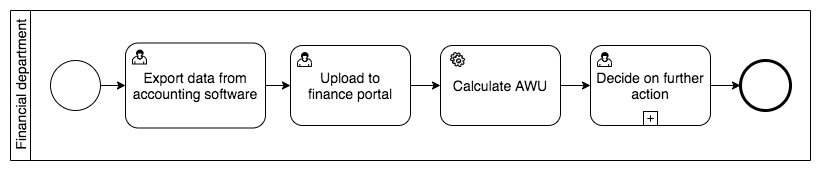
\includegraphics[width=\textwidth]{after_automation.png}
        \caption{Process after automation}
        \label{fig:after_automation}
    \end{figure}
    
    
    \section{Input data}
    In order to be able to work with the data, we first need to be able to 
    The employee data is gathered from an accounting system and exported in an excel file. The table below shows how the data is structured.
    
    While there is some room for adjustments when it comes to the structure of the data we will be processing, we want avoid doing any manual interventions as much as possible. Because of this, we agreed with the finance department on a specific data format.
    
    From our agreed upon data structure definition, 
    \begin{center}
    \begin{tabular}{ |c|c|c|c|c|c|c|c| } 
    \hline
    ID & Surname & Name & Type & January & February & ... & December \\
    \hline
    1 & Smetana & Bedřich & R & 1 & 1 & ... & 1\\ 
    2 & Janáček & Leoš & N & 0.5 & 1 & ... & 1\\ 
    3 & Karel & Borovský & R & 0.5 & 1 & ... & 1\\ 
    \hline
    \end{tabular}
    \end{center}
    Tady popíšu zabezpečení integrace, přenos dat a způsob synchronizace
    
    When designing systems integration, we don't need to reinvent the wheel. In fact, it is best if we choose some standard set by the industry. Like object oriented programming, systems integration also has it's design patterns and best practices. One such pattern is PATTERN GOES HERE
    
    -
    The goal of process optimization in general is to simplify the process as much as possible. This can be done by automating tasks that are being done manually or by removing them altogether.-
    
    
    
    \begin{figure}[H]
        \centering
        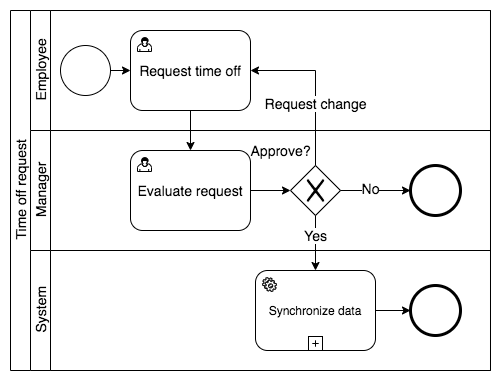
\includegraphics[width=\textwidth]{after_sys_integration.png}
        \caption{Process after system integration}
        \label{fig:after_sys_integration}
    \end{figure}
    
    To implement this integration, we can use our existing AWS infrastructure from our finance automation part. Here, we can create 
    
    First, we would create a lambda function that 
    
    \begin{figure}[H]
        \centering
        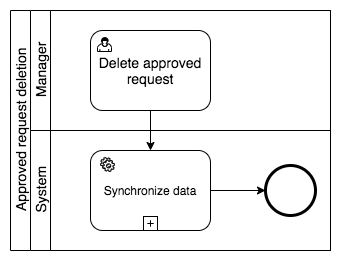
\includegraphics[width=0.6\textwidth]{delete_approved.png}
        \caption{Approved request deletion}
        \label{fig:delete_approved}
    \end{figure}
    
    
    \section{Technologies}
    The company is executing on it's mission to: "Innovate the way video-lovers discover, watch, and experience great content."\cite{24i-mission} by using the latest and greatest technologies that are available on the market. To build it's infrastructure and services, the company has chosen to use Amazon Web Services (AWS). Because of this, it only made sense to also use AWS in this thesis.
    The intent of this chapter is to provide a brief overview of the core technologies used in this thesis. More importantly, however, this list serves to demonstrate how these technologies have helped to achieve the thesis goals.
    Amazon Web Services (AWS) is a branch of Amazon Inc. that provides a cloud computing platform and a variety of APIs to a broad range of customers, including companies and individuals alike. In it's entirety, AWS provides a set of abstract technical infrastructure and distributed computing building blocks and tools. This helps companies create solutions faster, more easily and with a higher degree of cost efficiency. \cite{what-is-aws} Thanks to the distributed nature and pay-as-you-go billing schemes, it is a fast and cheap way of delivering a highly scalable solution. \cite{aws-pricing}
    \newline\newline
    The main reason for using AWS in this thesis are the pre-prepared building blocks that were used to assemble a secure website while maintaining low costs. Also, it is the ability to consume desired API services in order to provide value to the company.
    \subsection*{AWS Amplify}
    \subsection*{AWS Lambda}
    AWS Lambda is a serverless compute service that runs your code in response to events and automatically manages the underlying compute resources for you. You can use AWS Lambda to extend other AWS services with custom logic, or create your own back-end services that operate at AWS scale, performance, and security. AWS Lambda can automatically run code in response to multiple events, such as HTTP requests via Amazon API Gateway, modifications to objects in Amazon S3 buckets, table updates in Amazon DynamoDB, and state transitions in AWS Step Functions.
    \subsection*{AWS S3}
    \subsection*{AWS Cognito}
    \subsection*{React}
    React (also known as React.js or ReactJS) is an open-source, front end, JavaScript library for building application interfaces. It is maintained by Facebook and a community of individual developers and companies. React can be used as a base in the development of single-page or mobile applications. However, React is only concerned with rendering data to the DOM, and so creating React applications usually requires the use of additional libraries for state management and routing. Redux and React Router are respective examples of such libraries.
    \par
    I decided to use React to create the front end of the application mainly because I am using it every day as a part of my job, but also for it's ease of use and the ability to quickly develop a user interface.
    \subsection*{GatsbyJS}
    When used with React and GraphQL, GatsbyJS is a great tool for building web applications. Even though I am not using GraphQL I stil chose to use GatsbyJS, because it provides a variety of different starters to help get a site up and running quickly.
    \subsection*{TypeScript}
    The reasons to use TypeScript are similar to the ones I had for choosing React. TypeScript makes development in JavaScript more enjoyable, as it provides control over data types and introduces classes and interfaces. It is also a part of my work at the company.
    
    In such a dynamic and ever changing environment, which information technology undoubtedly is, more and more companies are placing their emphasis on security, robustness and scalability of their IT systems. These are some of the attributes, which can be attained by migrating data to and consuming computational power from a cloud based solution thanks to it's distributed and modular architecture.
    \par
    When thinking about system design, architects have to have a sense of complexity.
    \par
    In the first part of this chapter, an overview of the technologies used to create the application is presented. In the second part, the overall architecture of the system is described.
    \chapter{Implementation}
    In this chapter, we will describe the implementation. The process can be divided into four main sections:
    
    Web application
    Infrastructure
    Data storage
    Data manipulation
    
    vložit kódy a popsat, co konkrétně která část kódu řeší za problém

    Picking the right tools for the job
    Because we are creating an application that is both front-facing and back-end oriented at the same time, it is important that we choose technologies that are mature and up to date.
    When it comes to creating user interfaces, the ease of use and simplicity is very important both for the user and the developer. Because of this, I chose to use AWS Amplify in combination with GatsbyJS and React. Together, these three technologies make up the core of the front-end application. Amplify provides the infrastructure, GatsbyJS the routing and site generation and React ties it all together.
    
    \section{Web application}
    As we have already established, the main goal of this thesis is to automate a process of caltulating the AWU. To achieve this goal, we first need to be able to gather the data from the financial department. We will do this by providing them with a web application that fulfills all of the functional requirements described in the analysis.
    To accommodate for user authentication, we leverage 
    
    \subsection{}
    \subsection{Uploading a file}
    Together with collecting the data in a file, we also need to collect some additional information about the data. Specifically, to which company and what year does the data correspond to. To do this, we

    \section{Data transformation}
    To 
    Even though the format transformation from .xlsx to .csv file has introduced some additional code complexity, the decision to do so has proved to be a good one, as the read speed of dataframe outpace the dataframe.readExcel almost eightfold. \cite{csv-read-speed}
    \subsection{Storing the data}
    After 
    \subsection{Retrieving AWU}
    \begin{center}
    \begin{tabular}{ |c|c|c|c|c| } 
    \hline
    Period & R & N & N > 2 & 1 year R average \\
    \hline
    january/2017 & 14 & 1.75 & false & - \\
    \dots & \dots & \dots & \dots & \dots \\
    december/2017 & 15 & 2.75 & true & - \\
    january/2018 & 14 & 1.75 & false & 14.15833 \\
    \dots & \dots & \dots & \dots & \dots \\
    \hline
    \end{tabular}
    \end{center}
    \section{Future development}
    
    \chapter{Conclusion}
    The goal of this thesis was to create an application that would automate specific process. Also, to analyze the possibilities of integrating two systems. These goals stem from specific needs of a private company, therefore we examine the current state and gather project requirements. Based on the collection of requirements we propose and implement a solution. Finally, we evaluate the added value of our solution.
    \bibliographystyle{unsrt}
    \bibliography{thebibliography}
    \listoffigures
\end{document}
